\documentclass[a4paper,12pt,final, openany, titlepage, twoside]{book}

%permette di aggiungere altri pacchetti dai file inclusi
\usepackage[subpreambles]{standalone} 

%impostazioni lingua
\usepackage[T1]{fontenc}
\usepackage[utf8]{inputenc}
\usepackage[english,italian]{babel}

%sistema i margini
\usepackage{geometry}
\geometry{a4paper,top=2.2cm,bottom=2.2cm,left=3cm,right=3cm, heightrounded}

%interlinea 1.5
\usepackage{setspace}
\onehalfspacing

%gestione delle testatine
\usepackage{fancyhdr}
\pagestyle{fancy}
\lhead{}
\chead{}
\rhead{TITOLO}
\lfoot{}
\cfoot{\thepage}
\rfoot{}
\renewcommand{\headrulewidth}{0.4pt}

%formattazione titoli paragrafo
\usepackage{titlesec}
\titleformat{\chapter}[block]{\normalfont\huge\bfseries}{\thechapter.}{0.7em}{\huge}


\usepackage[autostyle,italian=guillemets]{csquotes}
\usepackage[sorting=none,style=numeric,citestyle=numeric-comp,backend=biber]{biblatex}

\addbibresource{bibliografia.bib}

%collegamenti ipertestuali
%\usepackage{hyperref}

%genera testo casuale
\usepackage{lipsum}

\begin{document}
	
	
	\frontmatter
	\documentclass[crop=false]{standalone}

\usepackage{frontespizio}

\begin{document}
	\begin{frontespizio}
		\Preambolo{\renewcommand{\fronttitlefont}{%
				\fontsize{22}{22}\bfseries}}
		
		\Universita{Padova}
		\Logo[3cm]{./resources/images/loghi.jpg}
		\Dipartimento{Ingegneria dell'Informazione}
		\Corso[Laurea]{Ingegneria Informatica}
		\Titolo{Google ARCore}
		%aggiunge più candidati
		\NCandidati{}
		%elimina il carattere ":"
		\Punteggiatura{}
		\Preambolo{\renewcommand{\frontcandidatesep}{0.5cm}}
		\Candidato[1216433]{Marco Vettore}
		\Candidato[1227153]{Alberto Varini}
		\Candidato[1219603]{Mattia Tamiazzo}
		\Rientro{1cm}
		\Annoaccademico{2021-2022}
		\Margini{1.5cm}{1cm}{1.5cm}{1cm}
	\end{frontespizio}
\end{document}

	\documentclass[crop=false]{standalone}

\begin{document}
	\tableofcontents
\end{document}
	
	
	\mainmatter
	\documentclass[crop=false, class=book]{standalone}

%impostazioni lingua
\usepackage[T1]{fontenc}
\usepackage[utf8]{inputenc}
\usepackage[english,italian]{babel}

%sistema i margini
\usepackage{geometry}
\geometry{a4paper,top=2.2cm,bottom=2.2cm,left=3cm,right=3cm, heightrounded}

%interlinea 1.5
\usepackage{setspace}
\onehalfspacing

%gestione delle testatine
\usepackage{fancyhdr}
\pagestyle{fancy}
\lhead{}
\chead{}
\rhead{Titolo}
\lfoot{}
\cfoot{\thepage}
\rfoot{}
\renewcommand{\headrulewidth}{0.4pt}

%formattazione titoli paragrafo
\usepackage{titlesec}
\titleformat{\chapter}[block]{\normalfont\huge\bfseries}{\thechapter.}{0.7em}{\huge}

%pacchetti per i riferimenti in bibliografia
\usepackage[autostyle,italian=guillemets]{csquotes}
\usepackage[sorting=none,style=numeric,citestyle=numeric-comp,backend=biber]{biblatex}

%risorsa che contiene la bibliografia
\addbibresource{./../bibliografia.bib}



\begin{document}
	\chapter{Introduzione}
	La Realtà Aumentata (Augmented Reality - \emph{AR}) è una tecnologia che permette di compiere esperienze interattive, in cui l'ambiente reale viene arricchito da contenuti virtuali. Similmente alla realtà virtuale, vengono creati elementi grafici sintetici con cui l'utente può interagire attraverso i sensi. Tuttavia, come spiegato in \cite{bimber2005spatial}, nell'AR l'ambiente reale gioca un ruolo fondamentale: lo scopo della realtà aumentata è proprio cercare di collegare il mondo reale con quello virtuale.
	\\
	L'AR viene definita in \cite{azuma1997survey} come un sistema che incorpora tre caratteristiche principali: la combinazione tra reale e virtuale, l'interazione real-time e la rappresentazione 3D. 
	
	\section{Storia}
	Il primo rudimentale sistema di realtà aumentata è stato creato da Ivan Sutherland \cite{sutherland1968head} nel 1968. Esso era composto da un display ottico trasparente che veniva montato sulla testa e che poteva mostrare semplici immagini in tempo reale. Nel 1993 George Fitzmaurice ha creato \textit{Chameleon} \cite{fitzmaurice1993situated}, un dispositivo che tramite un piccolo schermo collegato a una videocamera poteva essere orientato per esplorare uno spazio virtuale 3D. Simile al prototipo di Fitzmaurice, nel 1995 Jun Rekimoto e Katashi Nagao creano \textit{NaviCam} \cite{rekimoto1995world}, che prendendo in input un flusso video poteva riconoscere in real-time dei marcatori colorati e sovrapporre al video delle informazioni testuali. 
	\\
	Dal 2000 vengono creati altri primi sistemi di realtà aumentata, con applicazioni soprattutto a giochi interattivi, come ad esempio l'estensione \textit{ARQuake} \cite{thomas2000arquake} o \textit{Human Pacman} \cite{cheok2003human}, ancora vincolati alle scarse prestazioni dei dispositivi mobili. Solo con l'aggiunta ai cellulari della fotocamera, e poi di schermi touch, vengono quindi create le prime applicazioni commerciali in grado di sfruttare le potenzialità della realtà aumentata. Ne sono esempi \textit{AR Tennis} \cite{henrysson2006ARtennis}, primo gioco in AR collaborativo per cellulare, e \textit{ARhrrrr!}, primo gioco mobile in realtà aumentata con contenuti grafici di alta qualità. Vengono quindi sviluppate le prime librerie software per la realtà aumentata, come \textit{ARToolKit}, implementata prima in linguaggio C e poi in C++ nelle versioni più recenti, \textit{OpenCV}, che possiede anche funzionalità per l'AR, e dal 2018 la libreria per Android \textit{ARCore} di Google.
	
	\section{Applicazioni}	
	Le applicazioni della realtà aumentata possono riguardare diversi ambiti, ai quali questa tecnologia può apportare benefici economici o qualitativi, oppure creare servizi innovativi \cite{carmigniani2011augmented}. 
	\\
	In particolare, nel corso degli anni la tecnologia AR è stata usata per scopi pubblicitari e commerciali, quali la prova di capi d'abbigliamento senza doverli indossare o l'integrazione al marketing cartaceo di video promozionali tramite riconoscimento delle immagini, o per l'intrattenimento, come nello sviluppo di videogiochi. Trova inoltre applicazioni nella produzione industriale, in cui vengono sovrapposte all'area di lavoro istruzioni virtuali, nell'ambito militare, come l'addestramento al volo dei piloti, o per la formazione e la pratica sanitaria.
\end{document}
	\documentclass[crop=false, class=book]{standalone}




\begin{document}
	\chapter{Realtà aumentata}
	La Realtà Aumentata (Augmented Reality - \emph{AR}) è una tecnologia che permette di compiere esperienze interattive, in cui l'ambiente reale viene arricchito da contenuti virtuali. Similmente alla realtà virtuale, vengono creati elementi grafici sintetici con cui l'utente può interagire attraverso i sensi. Tuttavia, come spiegato in \cite{bimber2005spatial}, nell'AR l'ambiente reale gioca un ruolo fondamentale: lo scopo della realtà aumentata è proprio cercare di collegare il mondo reale con quello virtuale.
	\\
	L'AR viene definita in \cite{azuma1997survey} come un sistema che incorpora tre caratteristiche principali: la combinazione tra reale e virtuale, l'interazione real-time e la rappresentazione 3D. 
	
	\section{Storia}
	Il primo rudimentale sistema di realtà aumentata è stato creato da Ivan Sutherland \cite{sutherland1968head} nel 1968. Esso era composto da un display ottico trasparente che veniva montato sulla testa e che poteva mostrare semplici immagini in tempo reale. Nel 1993 George Fitzmaurice ha creato \textit{Chameleon} \cite{fitzmaurice1993situated}, un dispositivo che tramite un piccolo schermo collegato a una videocamera poteva essere orientato per esplorare uno spazio virtuale 3D. Simile al prototipo di Fitzmaurice, nel 1995 Jun Rekimoto e Katashi Nagao creano \textit{NaviCam} \cite{rekimoto1995world}, che prendendo in input un flusso video poteva riconoscere in real-time dei marcatori colorati e sovrapporre al video delle informazioni testuali. 
	\\
	Dal 2000 vengono creati altri primi sistemi di realtà aumentata, con applicazioni soprattutto a giochi interattivi, come ad esempio l'estensione \textit{ARQuake} \cite{thomas2000arquake} o \textit{Human Pacman} \cite{cheok2003human}, ancora vincolati alle scarse prestazioni dei dispositivi mobili. Solo con l'aggiunta ai cellulari della fotocamera, e poi di schermi touch, vengono quindi create le prime applicazioni commerciali in grado di sfruttare le potenzialità della realtà aumentata. Ne sono esempi \textit{AR Tennis} \cite{henrysson2006ARtennis}, primo gioco in AR collaborativo per cellulare, e \textit{ARhrrrr!}, primo gioco mobile in realtà aumentata con contenuti grafici di alta qualità. Vengono quindi sviluppate le prime librerie software per la realtà aumentata, come \textit{ARToolKit}, implementata prima in linguaggio C e poi in C++ nelle versioni più recenti, \textit{OpenCV}, che possiede anche funzionalità per l'AR, e dal 2018 la libreria per Android \textit{ARCore} di Google.
	
	\section{Applicazioni}	
	Le applicazioni della realtà aumentata possono riguardare diversi ambiti, ai quali questa tecnologia può apportare benefici economici o qualitativi, oppure creare servizi innovativi \cite{carmigniani2011augmented}. 
	\\
	In particolare, nel corso degli anni la tecnologia AR è stata usata per scopi pubblicitari e commerciali, quali la prova di capi d'abbigliamento senza doverli indossare o l'integrazione al marketing cartaceo di video promozionali tramite riconoscimento delle immagini, o per l'intrattenimento, come nello sviluppo di videogiochi. Trova inoltre applicazioni nella produzione industriale, in cui vengono sovrapposte all'area di lavoro istruzioni virtuali, nell'ambito militare, come l'addestramento al volo dei piloti, o per la formazione e la pratica sanitaria.
	
	 
\end{document}
	
	\documentclass[crop=false, class=book]{standalone}


%pacchetto per immagini
\usepackage{graphicx}

\usepackage[italian]{varioref}
\usepackage{copyrightbox}
\usepackage{url}

\begin{document}
	\section{Light Estimation}
	\label{sec:light_est}
	Nel rendering in realtà aumentata è importante che gli oggetti virtuali siano il più possibile integrati con l'ambiente circostante. Una delle caratteristiche principali che permette all'occhio umano di percepire la posizione di un oggetto nello spazio è la luce, cioè il modo in cui esso viene illuminato e l'ombra che proietta. 
	Proprio per questo motivo, il framework ARCore mette a disposizione il \textit{Light Estimation API}, che fornisce informazioni dettagliate riguardo l'illuminazione della scena, come spiegato nella documentazione ufficiale \cite{google2022light}.
	Tali informazioni sono necessarie per imitare i vari effetti che producono gli oggetti reali quando colpiti da una fonte di luce, che sono descritti dalla figura~\vref{fig:light_effects}:
	\begin{itemize}
		\item le \textbf{ombre} (\textit{shadows}), che sono direzionali e suggeriscono dove è collocata la fonte di luce;
		\item l'\textbf{ombreggiatura} (\textit{shading}), cioè l'intensità della luce che colpisce una certa faccia dell'oggetto;
		\item la \textbf{lumeggiatura} (\textit{specular highlight}), la macchia luminosa che compare su un oggetto lucido quando viene illuminato;
		\item la \textbf{riflessione} (\textit{reflection}), che può essere con proprietà speculari per oggetti completamente lucidi, come ad esempio uno specchio, oppure di diffusione, non dando un chiaro riflesso dell'ambiente circostante. 
	\end{itemize}
	
	\begin{figure}
		\centering
		\copyrightbox[l]{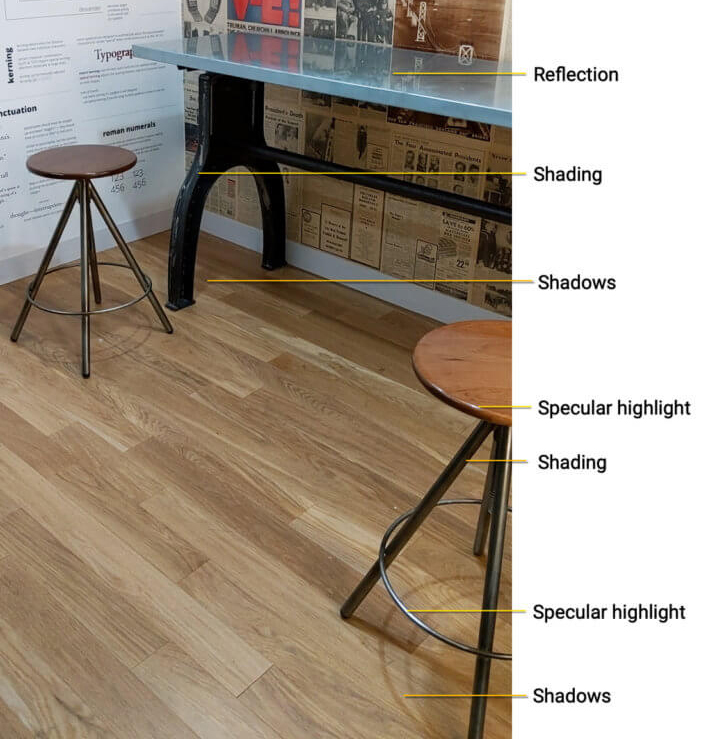
\includegraphics[width=0.5\textwidth]{./resources/images/light_estimation/light_effects}}%
			{Fonte: \url{https://developers.google.com}}
		\caption{Esempio degli effetti prodotti dagli oggetti quando sono illuminati.}
		\label{fig:light_effects}
	\end{figure}
    \noindent
	Le modalità per la gestione della stima della luce sono due, l'\textit{Environmental HDR mode} e l'\textit{Ambient intensity mode}. Durante la configurazione della sessione ARCore può essere scelta una delle due modalità, oppure disabilitare la stima della luce, come mostra il listing~\vref{lst:le_session} tratto dalla guida ufficiale.
	\\
	
	\begin{center}
		\begin{minipage}{0.95\textwidth}
			\begin{lstlisting}[caption={Configurazione della modalità di stima della luce.}, label={lst:le_session}, language=Kotlin]
			// Configura la sessione in modalità \verb|ENVIRONMENTAL_HDR|
			val config : Config = session.config
			config.lightEstimationMode = LightEstimationMode.ENVIRONMENTAL_HDR
			session.configure(config)
			
			// Configura la sessione in modalità \verb|AMBIENT_INTENSITY|
			val config : Config = session.config
			config.lightEstimationMode = LightEstimationMode.AMBIENT_INTENSITY
			session.configure(config)
				
			// Configura la sessione disabilitando la Light Estimation API
			val config : Config = session.config
			config.lightEstimationMode = LightEstimationMode.DISABLED
			session.configure(config)
			\end{lstlisting}
		\end{minipage}
	\end{center}


	

	\subsection{Environmental HDR mode}
		La modalità \textit{Environmental HDR} combina tre diverse API per replicare la luce reale, come descritti dalla figura~\vref{fig:env_HDR}.
	
		\paragraph*{Main Directional Light}
			Questa API calcola la direzione e l'intensità della fonte di luce principale, permettendo di posizionare correttamente l'ombra e la lumeggiatura dell'oggetto virtuale. Inoltre, questa funzionalità permette ad entrambi questi effetti ottici di venire corretti se cambia la posizione relativa dell'oggetto rispetto la fonte di luce
		
		\paragraph*{Ambient Spherical Harmonics}
			Questa funzionalità permette di rappresentare la luce ambientale della scena, parametrizzando l'intensità della luce proveniente dalle varie direzioni.
		
	
		\paragraph*{HDR Cubemap}
			Essa permette di riprodurre la riflessione di oggetti con superfici lucide. Tramite questa API viene modificata anche l'ombreggiatura e il colore dell'oggetto, che dipenderanno dalla tonalità dell'ambiente circostante.
	
		\begin{figure}
			\centering
			\copyrightbox[l]{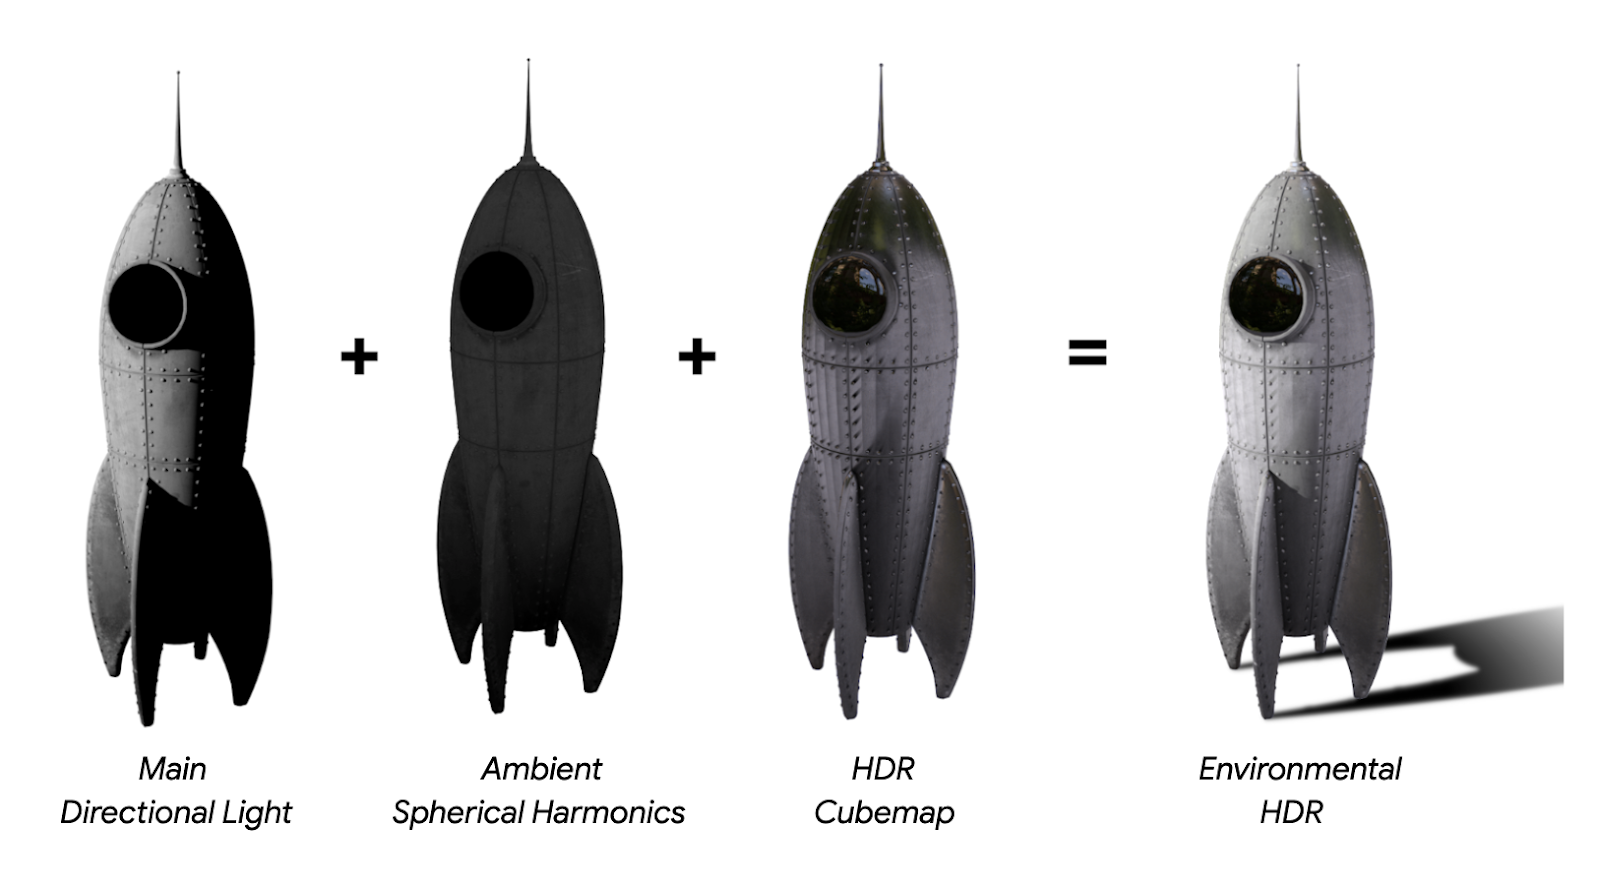
\includegraphics[width=0.8\textwidth]{./resources/images/light_estimation/env_HDR}}%
			{Fonte: \url{https://developers.googleblog.com}}
			\caption{Composizione della modalità Environmental HDR.}
			\label{fig:env_HDR}
		\end{figure}
	
	\subsection{Ambient intensity mode}
		La modalità \textit{Ambient intensity} determina l'intensità media dei pixel e la correzione del colore di una data immagine. Dopo aver filtrato l'intensità media di un insieme di pixel e il bilanciamento del bianco per ogni frame, vengono corretti la luce e il colore dell'oggetto virtuale, affinché si integri meglio con la scena \cite{suonsivu2020rgbd}. Questa modalità può essere utilizzata se la stima della luce non è critica, come per oggetti che possiedono già una propria illuminazione integrata.
	
	
\end{document}
	
	
	\backmatter
	\documentclass[crop=false]{standalone}


\usepackage[autostyle,italian=guillemets]{csquotes}
\usepackage[style=numeric,citestyle=numeric-comp,backend=biber]{biblatex}

\addbibresource{bibliografia.bib}

\begin{document}
	\printbibliography[heading=bibintoc]
\end{document}
	
	
\end{document}
